\documentclass[10pt]{article}
\usepackage[final]{graphicx}
%\usepackage{graphicx}
\usepackage{float}
\usepackage[caption = false]{subfig}
\usepackage{amsmath,amssymb}
\textheight 240mm
\textwidth  170mm
\oddsidemargin  0mm
\evensidemargin 0mm
\topmargin -20mm



\begin{document}                                       
%_________________________________________________________________
\title{Bacterial Electrophysiology: Initial explorations of Measurement Data}
\author{Prasanth Prahladan}
\maketitle

%_________________________________________________________________
\section{Introduction}


%_________________________________________________________________
\section{High-Dimensional Data Analysis}

A time-series (one trace from the database) comprising of n-time samples can be considered to be an n-dimensional vector. The longer the time-duration, the larger the dimension of the space of representing a data-point. Further, our measurement system and observations can only permit us to sample a very small/finite number of data-points in that very large-dimensional data-space. Therefore, the analysis of this dataset would require we apply advanced algorithms, that are applicable to this domain of inquiry and research. 

In this section, we intend to apply concepts from High-Dimensional data-analysis for the purpose of mining patterns in the dataset and hopefully predict and extract information about the biophysical processes that constitute the lifetime of a Bacteria. We adopt the following architectural-framework for guiding our choice of methods, in the analysis of high-dimensional datasets. 
\begin{enumerate}
\item Embedding of Dataset into a Metric Space:\\
It is important to note that the representation of data-files in memory, needs to be chosen based on the application for which that data shall be utilized.For the purpose of classification, we need to design/develop a particular vector-representation that incorporates certain "descriptive features" of the traces. These "features" may be based on analytical notions of time-frequency domain representation. The representation of these features, as mathematical vectors embedded in a high-dimensional space, then permits us to use algorithms for processing vectorial data, for the purpose of automated classification/clustering. We intend to use the "spectrogram coefficients" and possibly other "high-level-feature" information for each of the trace files. 

\item Visual Pattern Detection of Biophysical Trace-Database: \\
The preliminary step involves the use of a Data-visualization library, to determine whether there are any patterns like clusters in the data, which can then be exploited. It would be helpful to understand the logic/ideas behind the algorithms used to guide the visualization process, which could then be incorporated into the classification engine, that we need to develop. 

\item Determine Intrinsic Dimension of the Data:\\
If any patterns(clusters) have been detected in the data-visualization, it helps to assume that the different genres of high-dimensional data in fact is distributed along low-dimensional manifolds embedded within the high-dimensional space. We can then use algorithms for determining the intrinsic dimension of these manifolds (e.g "Correlation Dimension" ). By determining the intrinsic-dimension of each of the genres, we can determine the minimum dimension of the space into which all the data can be embedded without losing much information. 

\item Metric Learning:\\
Ideally, when data are categorized into categories, we would like to believe that the traces/data-points that are "similar" to each other are "closer" to each other, and those that are "dissimilar" are "farther" apart. The closeness of two data-points is determined by the "distance metric" used to compute the distance between the two points. The reason such a "metric" would exist, can be deduced from the fact that the data points are distributed upon a Manifold. The measure of distance between any two points, thus becomes the distance travelled along the manifold surface between the points, rather than the shortest euclidean straight-line distance between them. The "metric-learning" problem deals with the problem of ascertaining the metric for each of the manifolds separately, or the notion of a "global-metric" for all the data-points.

\item Dimension Reduction:\\
Once the minimal intrinsic dimension of the datasets has been determined, and we have a notion of "distance-metric" that helps compute the distances between the points, we then deal with the problem of reducing the dimension of the data. We note that this procedure, helps us determine how much of the information from the initial choice of vector representation of the dataset is redundant. The solution to this problem, is the design of a Map/function that projects every data-point from the high-dimensional space to the low-dimensional space. To ensure that the representation for each data-point is unique in the reduced dimension, we impose the constraint of an injective mapping, on this function. 


\item Clustering:\\
If we have identified patterns in the data-visualization stage, we would assume that the traces belonging to the same music-genre are distributed as clusters in the high-dimensional space. We expect that the dimension-reduction process does not hamper/destroy the clustering of the dataset, but rather reinforce/amplifies the extent of clustering - "similar" traces are brought closer together and "dissimilar" traces are pushed farther apart. It is obvious that the "distance-metric" used to measure the distances between traces in the reduced-dimensional space is very-different from that in the high-dimensional space. However, we can demand that the distance metric in the reduced-space be closer to the Euclidean space. The "metric" in the reduced-space shall then be used to identify clusters in the dataset. 

\item Query Processing (Cluster Assignment/Statistical Learning):\\
Once the abstract model - a spatial distribution/representation of the traces in the database has been determined, we have now developed the capacity to determine the genre/family that a particular trace-query might belong to. We can develop a method to determine different classes representing differentiation within species of bacteria, by determining the cluster that it belongs to, the proximity to its neighbours and the classification of its neighbours into the different classes. 
\end{enumerate}

%_________________________________________________________________
\subsubsection{Feature vector representation}

To derive content-based features representative of each trace, we would have to implement digital signal-processing algorithms upon the .wav trace files, to compute quantitative information from each trace. Features extracted could be based on time-domain, frequency-domain or time-frequency domain. In this section, we focus on using the Spectral Information of the traces- represented by the spectrogram, to serve as the primary signature of a window-frame. 
Traces are thus analysed by using moving window of short-time duration. The window-length is arbitrarily chosen.
To further, obtain a compact representation of the features, we proceed to develop a code-word histogram representation of each trace. (Dis)Similarity between the traces is then measured in the vector space of this final reduced feature-vector representation. 


\paragraph{Code-word Histogram}
The code-word histogram \cite{codewordHist} approach to feature-vector representation of a trace can be described intuitively as follows. All the traces in the database can be assumed to be 'sentences' that are made up of a fixed number of 'code-words' in the vocabulary of bacterial inter-cellular electrical signals. Each trace is represented by the number of times specific 'code-words' occur in it. The word-histogram is used to describe this method of counting the number of times a given code-word occurs in the trace. Thus, by assuming such a finite word vocabulary to describe all possible traces in the database, we enable a  mechanism of drawing parallels between comparison of textual-documents via Natural-Language processing algorithms, and the analysis of biophysical signals. 

Mathematically, the code-word histogram generation process can be described as follows. To obtain a compact summary of bacterial electrical traces, each trace is represented as a histogram over a dictionary of codewords. As a first step, a codebook is constructed by clustering a large collection of feature-descriptors. Once the codebook has been constructed, each trace is summarized by aggregating vector-quantization representations across all frames in the trace, resulting in codeword histograms. Finally, histograms are represented in a nonlinear kernel space to facilitate better learning of the distance metric between the traces. 

\paragraph{Codebook training}
The primary spectral-feature descriptor used for training of the codebook, is the spectrogram coefficients of frames of a trace. The spectral-feature descriptors of all the traces in the database is aggregated into a single bag-of-features, which is then clustered to produce the codebook. In our implementation, the number of words in the codeword dictionary is arbitrarily chosen to be about 512. 

For each trace $x$(of length []s) in the codebook training set $X_C$, we compute the spectrogram coefficients from each overlapping []ms frame. These descriptors are then aggregated across all $x \in X_C$ to form an unordered bag of features $Z$, where each $ z \in Z \subset \mathcal{R}^D $ is either an spectrogram feature-vector representation of the trace-frames.

To correct for changes in scale across different dimensions of $ z \in Z$, each vector is normalized according to the sample mean $\mu \in \mathcal{R}^D$ and standard deviation $\sigma \in \mathcal{R}^D$ estimated from $Z$. The i'th coordinate is mapped by
\begin{align}
z[i] \mapsto \frac{z[i] - \mu[i]}{\sigma[i]}. \label{eq:NormlizeSPECG}
\end{align}The normalized feature vectors are then clustered into a set $\mathcal{V}$ of $|V| = 512$ codewords by k-means algorithm.

\paragraph{(Top $\tau$) Vector Quantization}
Once the codebook $\mathcal{V}$ has been constructed, a trace $x \in X_C$, is represented as a histogram $h_x$ over the codewords in the codebook. Each trace $x \in X_C$ is understood to be a time-sequence of feature-vectors, $ z = {z_i} \in Z \subset \mathcal{R}^D$ where $z_i$ is the feature-vector representation of a frame in the trace. Each $ z_i \in z$ is normalized according to \eqref{eq:NormlizeSPECG}. The codeword histogram of trace $x \in X_C$ is constructed by counting the frequency with which each codeword $v \in \mathcal{V}$ quantizes the elements of $z$ i.e
\begin{align}
h_x[v] = \frac{1}{|z|} \sum_{z_i \in z} \frac{1}{\tau}\i\bigg\lbrace v = arg\min_{u \in \mathcal{V}}^{\tau}||z_i - u|| \bigg\rbrace. \label{eq:wc_Hist_Defn}
\end{align}
where we have chosen to adopt multiple codeword quantizers of each vector $z_i$ by defining the quantization set
\begin{align}
arg\min_{u \in \mathcal{V}}^{\tau} = \big\lbrace u \text{ is a } \tau \text{-nearest neighbor of }z_i \big\rbrace. \label{eq:TauQuantize}
\end{align}
where $\tau \in {1,2,\cdots, |V|}.$
Note that the codeword histograms are normalized by the number of frames $|z|$ in the trace in order to ensure comparability between traces of different lengths. Further, the normalization by $1/\tau$ ensures that $\sum_v h_x^{\tau}[v] = 1$, so that for $\tau > 1$, $h_x^{\tau}$ retains its interpretation as a multinomial distribution over $\mathcal{V}$.


%_________________________________________________________________
\subsection{Distance and Similarity in trace-space}

The choice of the Distance-Metric depends on the chosen Feature-Vector-representation for each trace. The naive method to proceed would be to assume that all the traces are embedded in an Euclidean Space, and hence the distances can be computed using the L-2 Norm. However, for the specialized representations of the traces that we have adopted, we believe that the traces are distributed over a manifold, and hence the distance between the points need to be computed by using a metric intrinsic to that manifold. One approach would be to use metric-learning algorithms to learn the metric between the data points. 

Conventional choices of the distance measure between the traces(high-dimensional dataset) are:
\begin{enumerate}
\item Euclidean Distance\\
One can treat each n-sampled trace as a n-dimensional vector and then compute the euclidean distance of the same from another trace.
\item Cosine Distance\\
One method to determine the distance between the traces, is to compute the Correlation Matrix between them. For any pair i,j of traces, we compute the cosine of the angle between them, by computing the inner-product of the normalized traces. 
\end{enumerate}

\subsubsection{Similarity between traces in trace-space}
The distance matrix computed above can further be processed by choosing a particular threshold value. We determine the adjacency matrix of the graph, representing the relationship/relatedness between the traces. The graph-based path-distance between the traces, gives a measure of the similarity between the traces. Graph based methods for dimensional reduction can then be pursued for the given dataset. 

When using only the distance information to describe similarity, we can choose the function to be any number of non-linear functions like:
\begin{enumerate}
\item Thresholding $s_{ij} = \i[d_{ij} > \theta]$, where $\theta$ is chosen threshold value.
\item Gaussian Similarity $s_{ij} = exp(-d_{ij}^2 / 2\sigma)$,
\item Inverse distance $s_{ij} = \frac{1}{1 + d_{ij}^p}$, where $p \geq 1$,etc.
\end{enumerate}
We use the Similarity Matrices computed above, as inputs to some of the nonlinear dimension reduction techniques like the Refined-Graph-Embedding.

%_________________________________________________________________
\subsection{Data Visualization}
The t-SNE algorithm \cite{tSNEdataViz} is an award-winning algorithm, for visualizing high-dimensional datasets. We shall first implement this algorithm, to determine a possible visual representation of the database, that shall indicate visual patterns in the data. This visualization shall help us develop an intuition of what the data distributions might look like. 

This algorithm provides us the opportunity to check the efficiency of the vector-space embedding of the selected features from the traces in our database.  If the visualization does not separate our vector-space data set into a sufficient number of discrete clusters, then it is likely that our choice of features is inadequate to truly separate the different genres when implementing our own dimension reduction techniques.  In this case we will augment the vector-space embedding by adding additional features from the traces.  This visualization algorithm can also be used after each stage of the pipeline to check that the information in our dataset has not been adversely deformed. Further, this algorithm can also be used a dimension-reduction technique, and shall be described in the appropriate section below.


%_________________________________________________________________
\subsection{Dimension reduction}
%_________________________________________________________________
We shall create and compare multiple pipelines for the dimensional reduction process. Both linear and non-linear graph based methods shall be explored. 

Non-linear, Graph-based Refined Embedding. This method builds a similarity graph, between all the datapoints, where the edge-weights are computed using a particular kernel function and distance-metric. From the similarity graph, we derive the Graph-Laplacian and follow the procedure of spectral embedding of this graph. The eigenvalues and the eigenvectors of the Graph Laplacian shall indicate the existence of the clusters. 



\subsubsection{Refined Graph Embedding}
The Refined Graph Embedding relies on theoretical concepts covered in Spectral Graph theory. Let $G(V,E)$, with $|V| = n$ and $|E| = m $, be an undirected graph without self-loops. Let $A$ be the adjacency matrix defined as $A_{ij} = \i[(i,j) \in E]$ and $D$ be the degree-matrix of the graph $D = diag(d_1, d_2, \cdots d_n)$ with $d_i = \sum_{i=1}^n A_{ij}$. We further define the following matrices
\begin{align}
\begin{array}{cc}
L = D-A & \text{combinatorial unnormalized graph Laplacian}\\
P = D^{-1}A & \text{markov probability transition matrix}\\
\mathcal{L} = I - D^{-1/2}*A*D^{1/2} & \text{normlaized graph laplacian}
\end{array}
\end{align}
The largest eigenvalues and the corresponding eigenvectors of $\mathcal{L}$ are computed. Next, a stationary probability distribution is computed for the Markov Chain transition matrix $P$. The coordinates of the point in the reduced dimensional-space are obtained from the eigenvectors and the stationary-probability distribution computed. 


\subsubsection{t-Distributed Stochastic Neighbour Embedding}
The t-SNE algorithm \cite{tSNEdataViz}, was introduced earlier as a technique for visualization of high-dimensional datasets, to built a visual intuition of the data-distribution. From the fact that local neighbourhood information of the data is preserved by the technique, it would serve as a useful dimensional reduction technique, and hence used this method as an alternative to the Graph Embedding Technique.

tSNE starts by converting the high-dimensional Euclidean distances between data points  into conditional probabilities that represent similarities. The similarity of data-point $x_j$ to $x_i$ is the conditional probability $p_{j|i}$ that $x_i$ would pick $x_j$ as a neighbour, if the neighbours were picked in proportion to their probability density under a Gaussian centred at $x_i$. Mathematically, the conditional probability is computed as
\begin{align}
p_{j|i} = \frac{exp( - d_{ij}^2/ 2\sigma_i^2)}{\sum_{k \ne i} exp( - d_{ik}^2/ 2\sigma_i^2)}\label{eq:prob_nbr_HD}
\end{align} where $\sigma_i$ is the variance of the Gaussian centred about $x_i$. Because, we are only interested  in modelling pairwise similarities, we set the value of $p_{i|i} = 0$.

Now, we assume that there's a particular projection operation that projects each of the traces $x_i$ to lower dimensional point $y_i$. For the low dimensional counterparts $y_i$ and $y_j$ of the high-dimensional points $x_i$ and $x_j$, we can compute the conditional probability, $q_{j|i}$ as 
\begin{align}
q_{j|i} = \frac{(1 + d_{ij}^2)^(-1)}{\sum_{k \ne i} (1 + d_{ik}^2)^(-1)}
\end{align}
where, we use a t-Student distribution with a single degree of freedom, instead of a Gaussian distribution about point $y_i$. This is because, it has the particularly nice property that $(1 + d_{ij}^2)^(-1)$ approaches an inverse-square law for large pairwise distances in the low-dimensional map. This makes the maps representation of the joint probabilities almost invariant to changes in scale of the map for points that are far apart. Which also implies that large clusters of points that are far apart interact in just the same way as individual points, so the optimization operates in the same way at all but the finest scales. 

If the projections correctly model the similarity of the points in the high dimensional space, then the conditional probabilities $p_{j|i} = q_{j|i}$. Motivated by this intuition, the tSNE algorithm aims to find a low-dimensional data representation that tries to minimize the mismatch between joint conditional probabilities P and Q.	A natural measure of the distance between two distributions is the Kulback Liebler-divergence. tSNE minimizes the KL-divergence between P and Q, via a gradient descent algorithm. The cost function is given by
\begin{align}
C = \sum_i KL(P_i || Q_i) = \sum_i \sum_j p_{j|i} log(\frac{p_{j|i}}{q_{j|i}})\label{eq:Cost_tSNE}
\end{align}
where it is assumed that $\sigma_i = \sigma$ for all data-points. 

The gradient of the Kullback-Liebler divergence between P and the t-Student based joint probability distirbution Q is given by
\begin{align}
\frac{\delta C}{\delta y_i} =  4 \sum_j (p_{ij} - q_{ij})(y_i - y_j)(1 + d_{ij}^2)^(-1)\label{eq:Grad_KL_tsne}
\end{align} where $d_{ij} = ||y_i - y_j||$

%_________________________________________________________________
\subsection{Results of Experiment: Codeword Histogram}

The plots of the experiments using the spectrogram-codeword-histogram methodology gives a visual representation of the distribution of the traces in the 3 dimensional space. 
[Explain the procedure of constructing code-word histogram.]

Visually, we identify the pipeline comprising of the following:
\begin{enumerate}
\item Code-word Histograms of the spectrograms
\item t-Distributed Stochastic Neighbourhood Embedding
\item Clustering 
\end{enumerate} 

\begin{figure}[h!]
\centering
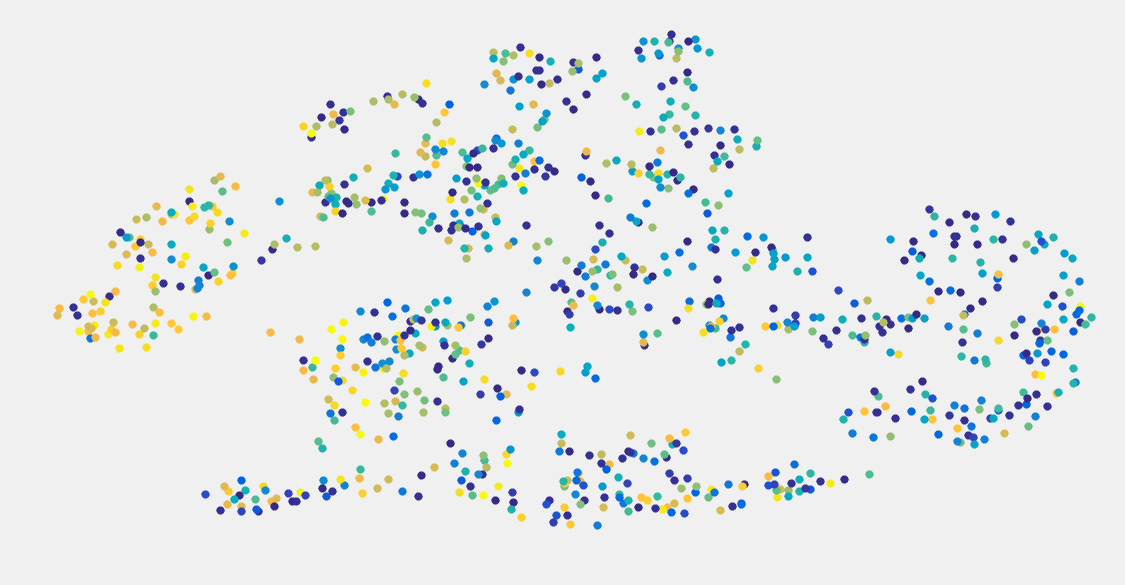
\includegraphics[scale=0.4]{cwHistogram_Components.png}\\
\caption{Plot of the traces categorized into classes based on graph components obtained by thresholding$(0.69)$ the correlation matrix.}
\label{fig:cwhist_specg_classes}
\end{figure}

\begin{figure}[h!]
\centering
\subfloat[time-series]{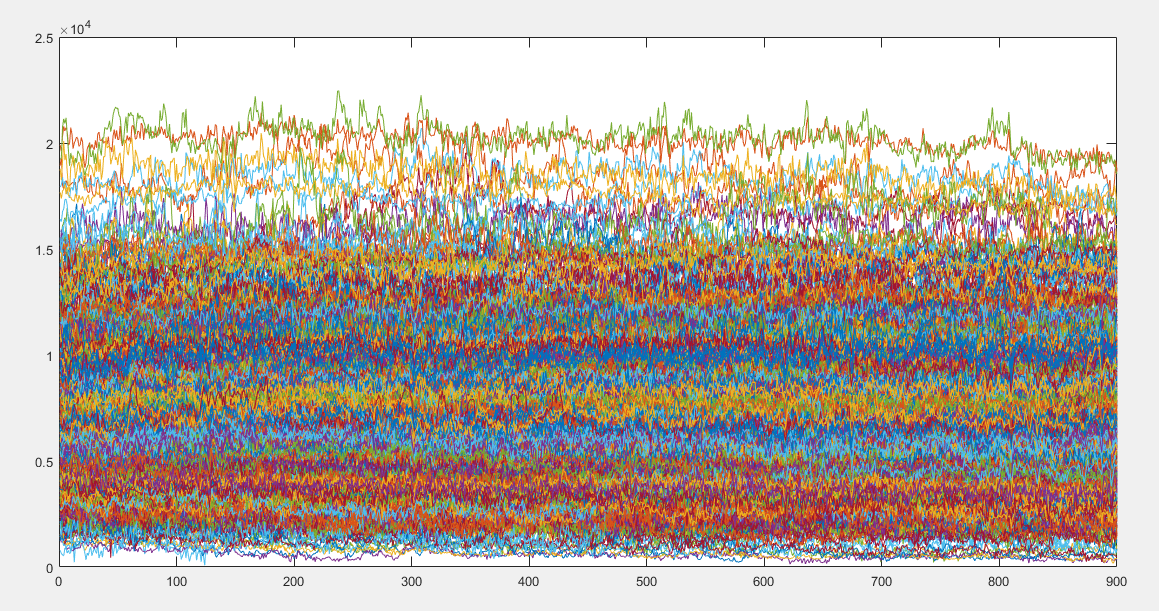
\includegraphics[scale=0.4]{allTraces_942.png}}\\
\subfloat[cw-histogram]{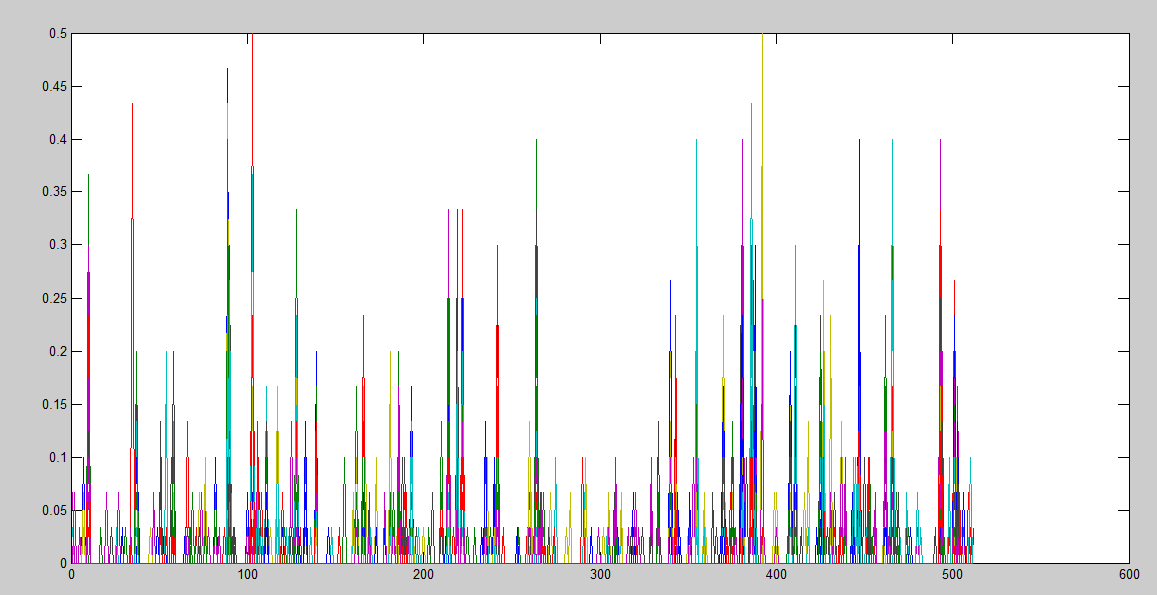
\includegraphics[scale=0.4]{queryPoints_cwHist.png}}\\
\caption{Plot of the traces when represented as (a)time-series dataset ;(b)code-word histograms based on choice of 512 codewords in "language".}
\label{fig:cwhist_allTraces}
\end{figure}





\pagebreak

%_________________________________________________________________
\section{1-Dimensional Time-series Analysis}

The time-series representation of the bacterial electrical signals, can be studied from the perspective of building linear or non-linear mathematical models of dynamical systems in high-dimensional spaces, who's trajectories in phase-space when projected onto a 1-dimensional manifold, provides us the traces measures. Else, we might pursue the analysis from a data-mining perspective, where we implement data-mining algorithms to detect motifs and patterns in the dataset. 

\subsection{Preliminary explorations}
We pursue our preliminary explorations on a database consisting of 942 time-series signals. Each traces corresponds to the observation/measurements from one bacteria, during the course of its life-process, while inhabiting a artificially life-supporting environment in the company of other individuals of the same or different microbial species.  
We can consider analysing each trace individually, to detect events and other "patterns", or we may look at all the traces as a multivariate time-series. 

We adopted the following methodology of probing into the dataset. First, we assume that there is no time-lag between the trace-signals from the bacteria. It might be possible that the source bacteria are communicating with each other. And since, we believe that they may communicate with each other, only via a chemical process, we would ideally expect there to be a delay in the transmission of signals from one cell to another. However, we ignore these aspects for the initial tests on the data, and hope to see if there's any patterns that's worth exploring. 

We compute the Correlation Matrix representing the cosine-distances between the traces by computing the inner-product of  the normalized traces. A value of 1 indicates identical signals and -1 indicates opposing signals. To identify the population of cells that might be communicating with each other(almost in synch with each other) we choose a particular threshold value($\theta$) and extract an Adjacency Matrix, representing the connectedness between correlated cells. 
We then generate the correlation-graph, $G(V,E)$ representing with V being the set of cells and E being the set of edges $\lbrace (i,j) \in E | CorrelationMatrix(i, j) \geq \theta  \rbrace$. A plot of the graph obtained, helps us identify the existence of a connected-components in the dataset. We extract the connected components from the graph by pursuing a depth-first search. Re-indexing the cells IDs by using the ordering obtained from a depth-first search, then helps us obtain a Correlation Matrix, in which the correlated components become visually self-evident. The cluster membership as determined by the depth-first search, can then be used to guide any other visualization scheme that we might wish to do, using the given dataset. 

Note that, at a threshold of 0.69 we obtain two large clusters, that are isolated from all other clusters. However, lower thresholds, have more inter-connectedness, and creates a Large-Connected-Component that links up a larger fraction of the population.
\begin{figure}[h!]
\centering
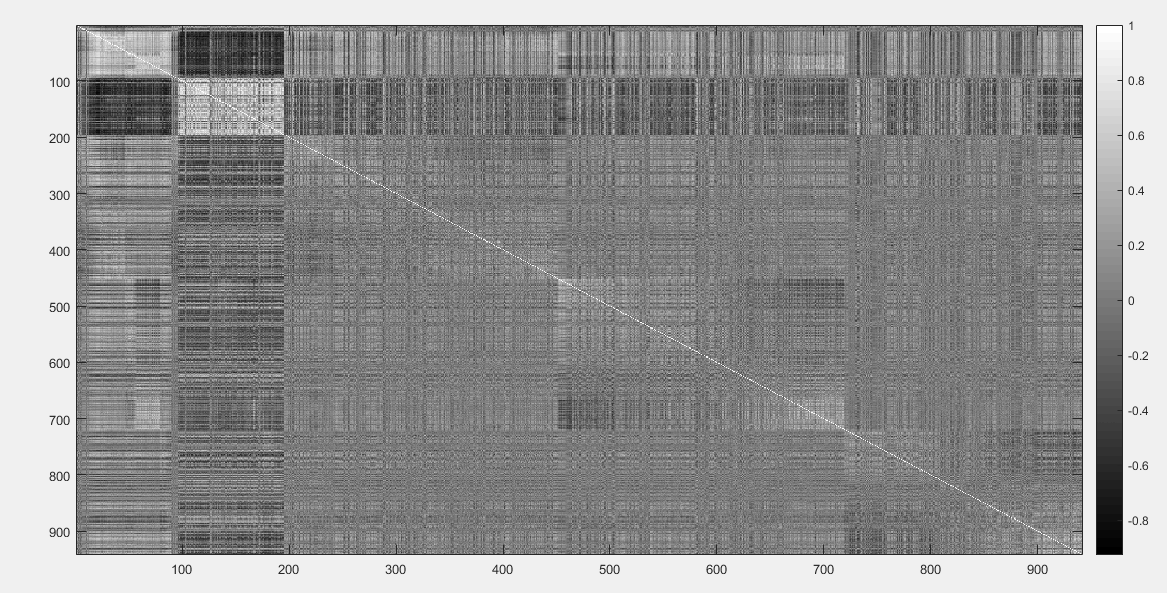
\includegraphics[scale=0.5]{components_CorrelationMatrix.png}
\caption{Determining connected components in correlation-matrix.}
\label{fig:correlationMatrix}
\end{figure}

Note that the cluster-membership histogram helps identify the distribution of the cells into components connected by high correlation index. 

\begin{figure}[h!]
\centering
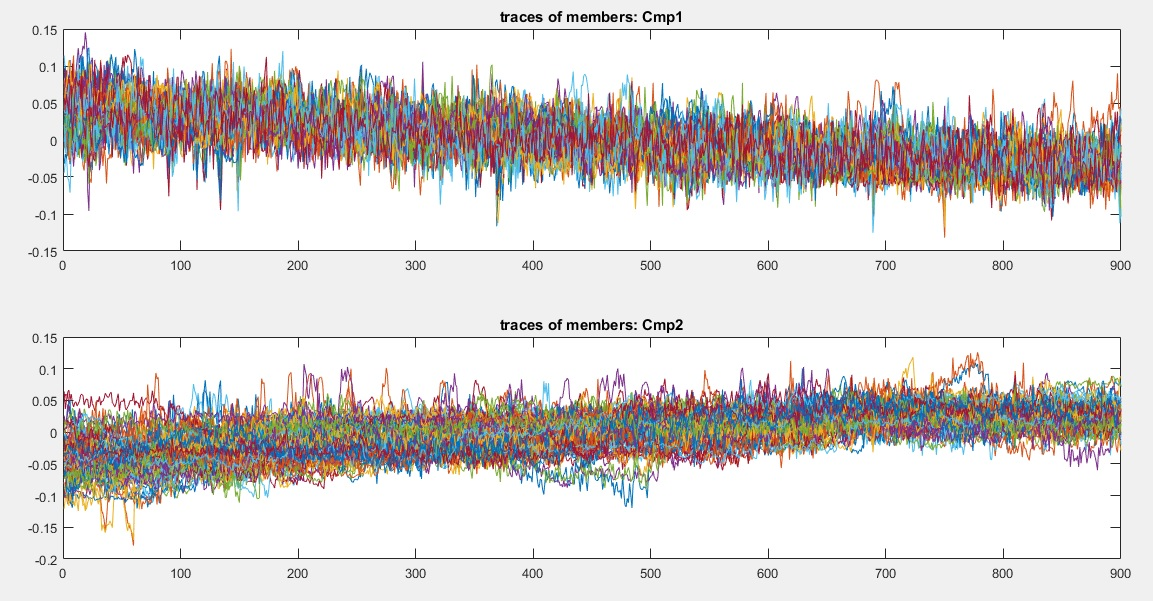
\includegraphics[scale=0.5]{component_traces.jpg}
\caption{Traces of cells in different components}
\label{fig:Traces_components}
\end{figure}


\begin{figure}[h!]
\centering
\subfloat[graphical components]{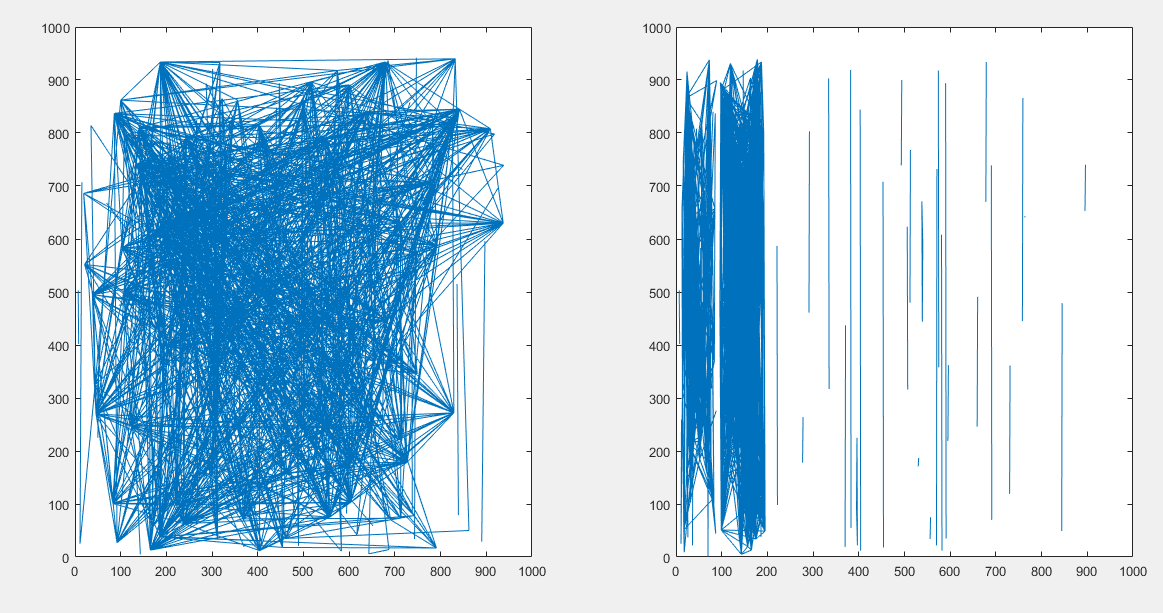
\includegraphics[scale=0.4]{components.png}}\\
\subfloat[correlation matrix]{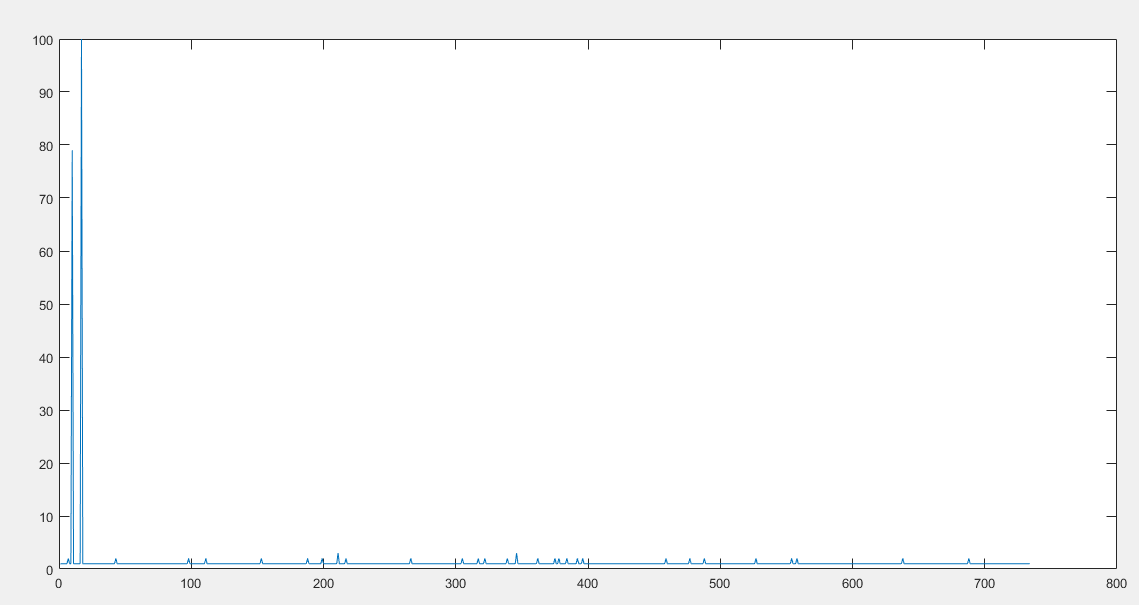
\includegraphics[scale=0.4]{membershipHistogram.png}}
\caption{Determining connected components in correlation-graph using threshold$ = 0.69$.}
\label{fig:cwhist_allTraces}
\end{figure}

The presence of connected components with members that are synchronized between themselves, but anti-symmetric with the members of the other component, is an extremely surprising observation in the dataset, given that we have assumed an absence of time-lags in the communication between the cells. 

This observation raises the following questions:
\begin{enumerate}
\item The high correlation value between the cells, indicates the presence of Synchrnoization between cells. Can we determine whether these cells were spatially located in each other's vicinity, or are there cells that are far away, but synchronized with each other?
\item Is it possible to determine the physical phenomena, by which synchronization at a distance might be realized?
\item Can we characterize the behaviour of the cells in each component? 
\end{enumerate}

\subsection{Analysis of synchronization between cells}
To analyze the synchronization between the cells, we first determine the average-trace representative of the behaviour of all the cells constituting a particular component. Further, we attempt to obtain a best-fit line that approximates the average-trace of each component. By computing the difference of each original trace from the average-signal and the best-fit curve, we can obtain the distribution of the noise in the recorded signals. It is interesting to observe that the noise-distribution has a uni-modal property \ref{fig:noises_components}.

These observations raise the following directions of research:
\begin{enumerate}
\item Is it possible to model the behaviour of the cells, as comprising of ramps and step-signals, with added noise.
\item Does the noise-statistics correspond to a Gaussian Distribution?
\end{enumerate}

\begin{figure}[h!]
\centering
\subfloat[avg-trace-1]{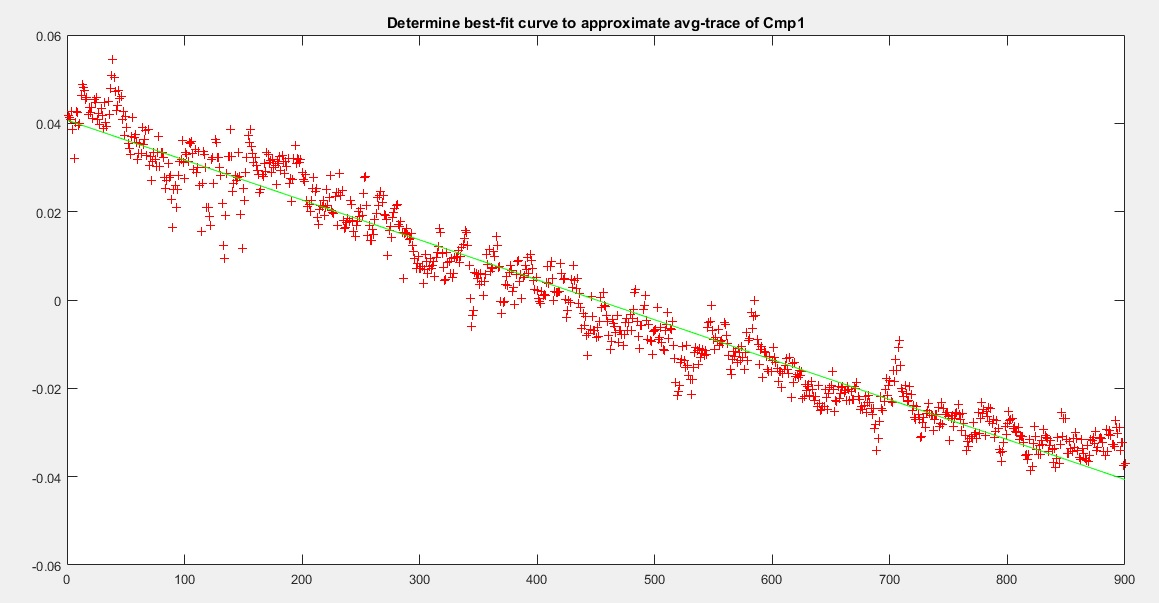
\includegraphics[scale=0.5]{bestFit_cmp1.jpg}}\\
\subfloat[avg-trace-2]{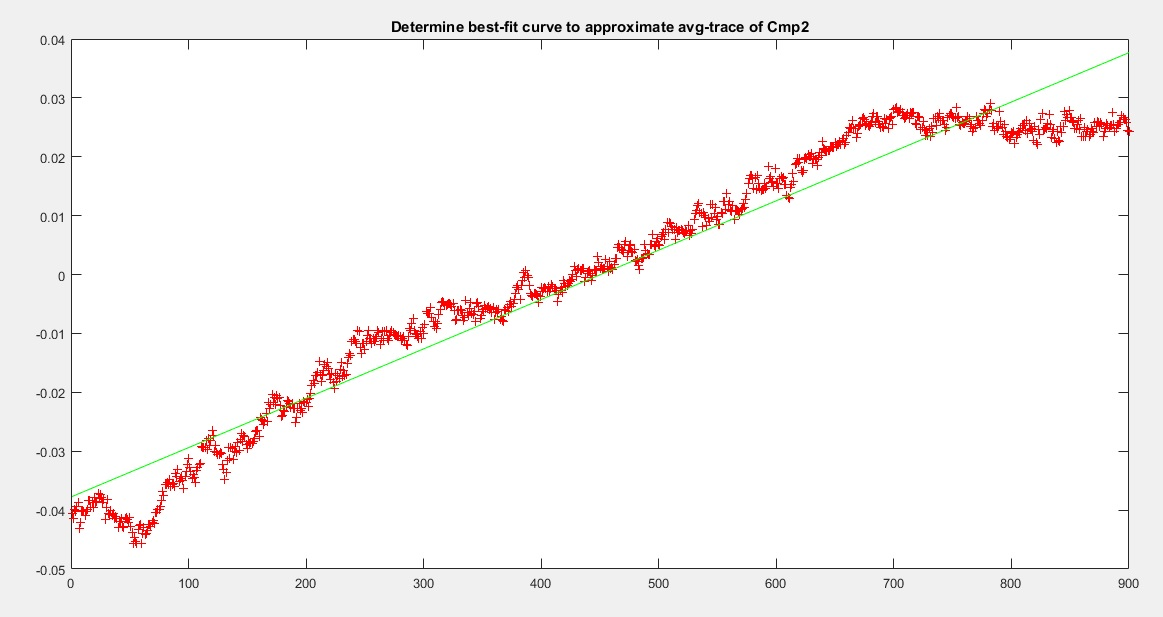
\includegraphics[scale=0.5]{bestFit_cmp2.jpg}}
\caption{(a)-(b) Average-Trace and Best-Fit trace, of cells in different components}
\label{fig:avgTraces_components}
\end{figure}


\begin{figure}[h!]
\centering
\subfloat[noise-from-avg]{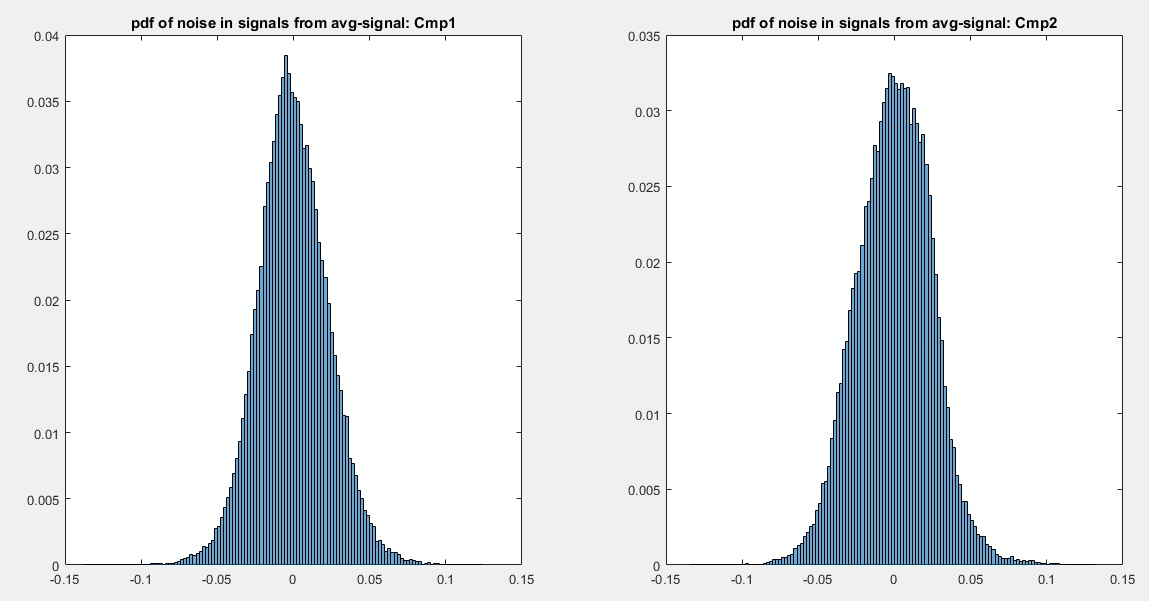
\includegraphics[scale=0.5]{component_noise_fromAvg.jpg}}\\
\subfloat[noise-from-bestFit]{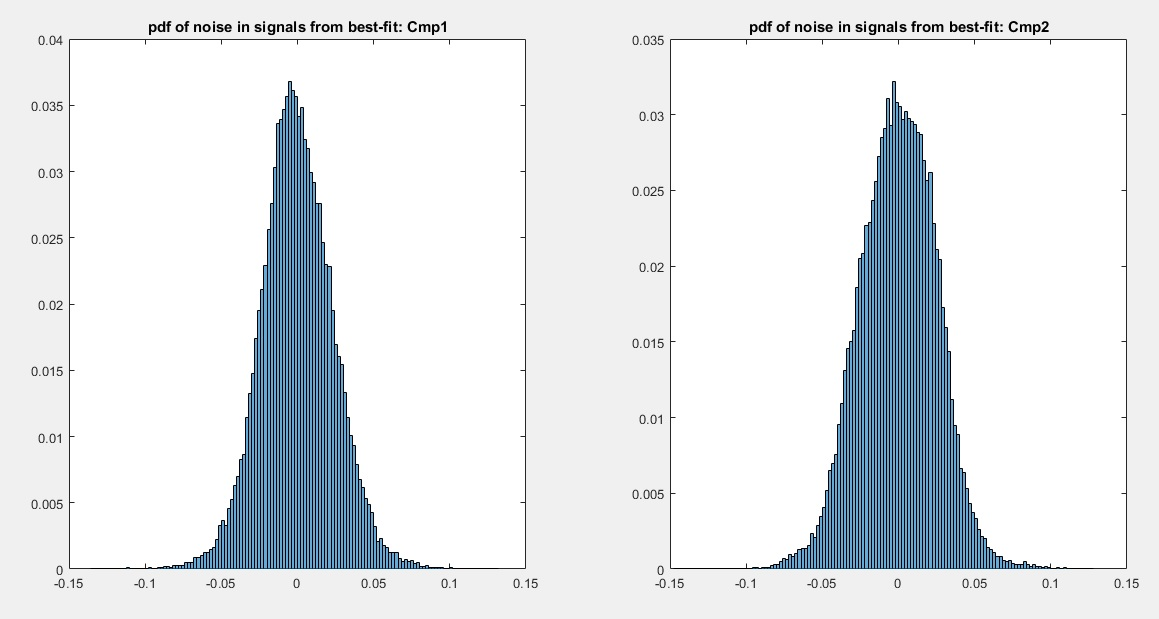
\includegraphics[scale=0.5]{component_noise_fromBestFit.jpg}}
\caption{Noise distribution in traces when compared to (a) Average-trace (b) Best-Fit-trace}
\label{fig:noises_components}
\end{figure}

\pagebreak



\pagebreak


%_________________________________________________________________
\section{Discussion}


%_________________________________________________________________
\begin{thebibliography}{5}

\bibitem{fjltAlgo}
\textit{Ailon, Nir and Chazelle, Bernard.} Faster Dimension Reduction, Communication of the ACM, Vol. 53, No. 2, February 2010;  doi:10.1145/1646353.1646379

\bibitem{infoTheoryMetricLearning}
\textit{Jason V. Davis, Brian Kulis, Prateek Jain, Suvrit Sra and Inderjit S. Dhillon.} Information Theoretic Metric Learning, ICML June 2007, 209-216,  http://www.cs.utexas.edu/~pjain/itml/

\bibitem{tSNEdataViz}
\textit{L.J.P. van der Maaten and G.E. Hinton.} Visualizing High-Dimensional Data Using t-SNE. Journal of Machine Learning Research 9(Nov):2579-2605, 2008, http://lvdmaaten.github.io/tsne/

\bibitem{intrinsicDims}
\textit{M. Hein, J.-Y. Audibert. }Intrinsic dimensionality estimation of submanifolds in Euclidean space,
In L. de Raedt and S. Wrobel, editors, Proceedings of the 22nd International Conference on Machine Learning (ICML 2005), 289 - 296, ACM press, 2005, http://www.ml.uni-saarland.de/publications.htm

\bibitem{fmeyer}
\textit{Non-normalized Laplacian on Weighted Graphs} http://ecee.colorado.edu/~fmeyer/class/ecen5322/laplacian.pdf

\end{thebibliography}

\section{Appendix}

\pagebreak


\end{document}


\begin{figure}[h!]
\subfloat[itml+tsne]{\includegraphics[scale=0.17]{spectrogram_itml_tsne_b01.jpg}}
\subfloat[tsne]{\includegraphics[scale=0.17]{spectrogramw_tsne.jpg}}\\
\subfloat[itml+graph]{\includegraphics[scale=0.17]{spectrogramw_itml_graph.jpg}}
\subfloat[graph]{\includegraphics[scale=0.17]{spectrogramw_graph.jpg}}
\caption{Plot of the structure of dataset obtained by using the following pipeline: spectrogram-code-word histogram features and (a)itml and tsne; (b) tsne alone; (c) imtl and graph embedding; (d) graph embedding alone.}
\label{fig:spectrogramw_dataview}
\end{figure}

\begin{figure}[h!]
\subfloat[S447 + raw-voting]{\includegraphics[scale=0.22]{BUNCH_test_trace_447_perbunch_raw.jpg}}
\subfloat[S447 + weighted-votes]{\includegraphics[scale=0.22]{BUNCH_test_trace_447_perbunch.jpg}}\\
\subfloat[S450 + raw-voting]{\includegraphics[scale=0.22]{BUNCH_test_trace_450_perbunch_raw.jpg}}
\subfloat[S450 + weighted-votes]{\includegraphics[scale=0.22]{BUNCH_test_trace_450_perbunch.jpg}}
\caption{Shows the votes per sample for each trace, showing only the votes for the known genre and the two other genres getting the most votes for this trace.}
\label{fig:fivesecond_trace_votes}
\end{figure}


\begin{figure}[h!]
\subfloat[S447 + raw-voting]{\includegraphics[scale=0.22]{BUNCH_test_trace_447_raw.jpg}}
\subfloat[S447 + weighted-votes]{\includegraphics[scale=0.22]{BUNCH_test_trace_447.jpg}}\\
\subfloat[S450 + raw-voting]{\includegraphics[scale=0.22]{BUNCH_test_trace_450_raw.jpg}}
\subfloat[S450 + weighted-votes]{\includegraphics[scale=0.22]{BUNCH_test_trace_450.jpg}}
\caption{Histogram bars show the sum of votes over all trace samples per genre.  Lines show the votes when assigning each sample to a genre.}
\label{fig:fivesecond_trace_histogram}
\end{figure}


\begin{figure}[h!]
\centering
\includegraphics[scale=0.4]{spectrogram_itml_tsne_b01.jpg}\\
\caption{Plot of the structure of dataset obtained by using a pipeline comprising of mfcc-code-word histogram features, itml and tsne.}
\label{fig:mfccw_itml_tsne}
\end{figure}



\begin{figure}[h!]
\subfloat[]{\includegraphics[scale=0.37]{jazzOutlier2.jpg}}
\subfloat[]{\includegraphics[scale=0.39]{jazzOutlier1.jpg}}
\caption{(a)Original distribution for 5-th nearest neighbour  distance for all jazz trace samples  (b) Retained distribution with outliers removed.}
\label{fig:jazz_outlier_removal}
\end{figure}

\begin{figure}[h!]
\centering
\includegraphics[scale=0.7]{comp_savings.jpg}
\caption{Computational savings from iterative outlier removal.}
\label{fig:compSavings}
\end{figure}



\begin{figure}[h!]
\centering
\includegraphics[scale=0.4]{FJLT_deformation.jpg}\\
\caption{FJLT Deformation}
\label{fig:fjlt_deformation}
\end{figure}
